\section{Deployment Considerations \& Recommendations}
\label{sec:deployment}
\textbf{External deployment.}
Following the one-time held-out evaluation, the final pipeline was applied without 
modification to the independent external dataset. The external data were not 
used for training, hyperparameter selection, threshold selection or testing.

The three required sensor streams were sampled at approximately 99.48~Hz,
consistent with the retained training recordings. After applying the same
signal derivation, operational-state gating, 4--46~Hz filtering, 2~s
windowing and 12-feature extraction procedure, 888 valid riding windows
remained.

The frozen RobustScaler and Logistic Regression model were then applied with
the previously selected threshold of 0.68. Figure~\ref{fig:deployment-prediction}
shows that most windows were predicted Smooth, interspersed with short
intervals where Bumpy probability exceeded the decision threshold.

\begin{figure}[htbp]
    \centering
    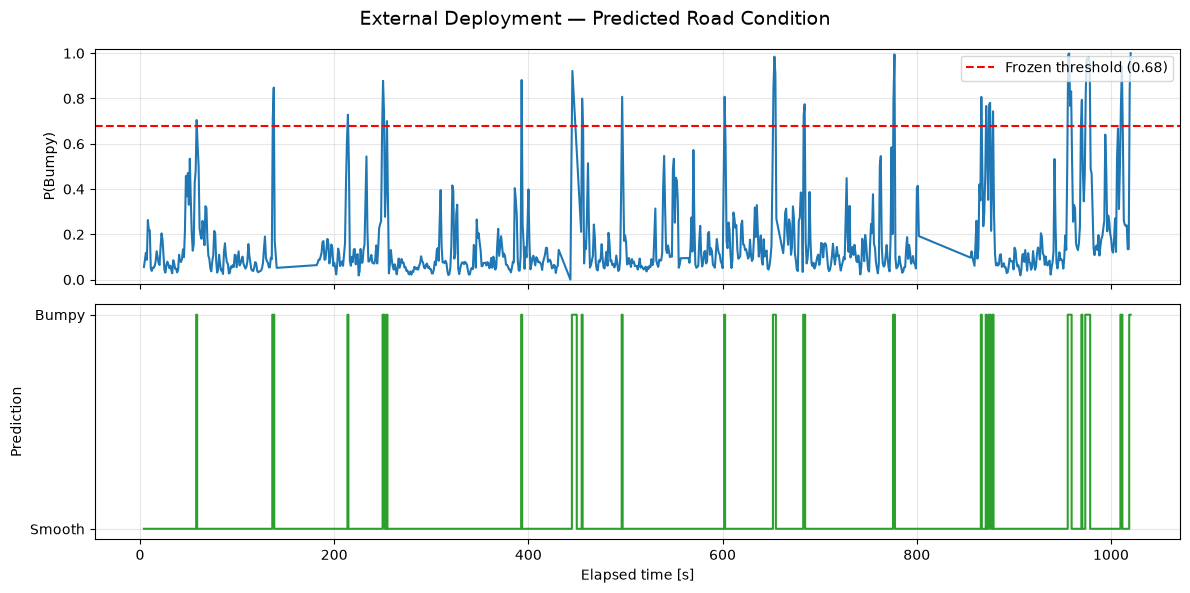
\includegraphics[width=0.9\linewidth]
    {figures/deployment-prediction.png}
    \caption{Deployment of the frozen Logistic Regression model on the
    independent external recording. The upper panel shows predicted Bumpy
    probability and the fixed threshold of 0.68; the lower panel shows the
    corresponding Smooth/Bumpy classification over elapsed time.}
    \label{fig:deployment-prediction}
\end{figure}

Because the external recording contains no terrain ground truth, these results
cannot be used to calculate classification performance. They instead
demonstrate that the complete preprocessing and inference pipeline can be
transferred to unseen sensor data and produce Smooth/Bumpy predictions over time, 
which would be suitable for a later stage real-time smartphone deployment.

\subsection{Limitations and Recommendations}

The main limitation is the small number of independent acquisition units.
Although 4246 valid windows were extracted, overlapping windows from the same
ride are correlated and should not be interpreted as independent experiments.
After participant~\#03 was excluded because of sampling-rate incompatibility,
only two participants remained.

The held-out results also indicate substantial recording-dependent
generalisation. In particular, the two unseen Bumpy recordings produced very
different outcomes: Raw022 achieved 87.5\% accuracy with mean Bumpy
probability 0.868, whereas Raw011 achieved only 11.6\% accuracy with mean
probability 0.414. Future data collection should therefore prioritise new
participants, devices, routes, riding speeds and acquisition sessions rather
than additional overlapping windows from existing rides.

A deployable implementation should also standardise a minimum sensor sampling
rate or redesign the spectral representation for devices unable to observe
the current 4--46~Hz band. Finally, the present preprocessing contains
offline/non-causal operations. Real-time smartphone deployment would require
causal filtering and explicit evaluation of latency, computational cost and
any resulting change in classification performance.